\documentclass[twoside]{book}

% Packages required by doxygen
\usepackage{fixltx2e}
\usepackage{calc}
\usepackage{doxygen}
\usepackage[export]{adjustbox} % also loads graphicx
\usepackage{graphicx}
\usepackage[utf8]{inputenc}
\usepackage{makeidx}
\usepackage{multicol}
\usepackage{multirow}
\PassOptionsToPackage{warn}{textcomp}
\usepackage{textcomp}
\usepackage[nointegrals]{wasysym}
\usepackage[table]{xcolor}

% Font selection
\usepackage[T1]{fontenc}
\usepackage[scaled=.90]{helvet}
\usepackage{courier}
\usepackage{amssymb}
\usepackage{sectsty}
\renewcommand{\familydefault}{\sfdefault}
\allsectionsfont{%
  \fontseries{bc}\selectfont%
  \color{darkgray}%
}
\renewcommand{\DoxyLabelFont}{%
  \fontseries{bc}\selectfont%
  \color{darkgray}%
}
\newcommand{\+}{\discretionary{\mbox{\scriptsize$\hookleftarrow$}}{}{}}

% Page & text layout
\usepackage{geometry}
\geometry{%
  a4paper,%
  top=2.5cm,%
  bottom=2.5cm,%
  left=2.5cm,%
  right=2.5cm%
}
\tolerance=750
\hfuzz=15pt
\hbadness=750
\setlength{\emergencystretch}{15pt}
\setlength{\parindent}{0cm}
\setlength{\parskip}{3ex plus 2ex minus 2ex}
\makeatletter
\renewcommand{\paragraph}{%
  \@startsection{paragraph}{4}{0ex}{-1.0ex}{1.0ex}{%
    \normalfont\normalsize\bfseries\SS@parafont%
  }%
}
\renewcommand{\subparagraph}{%
  \@startsection{subparagraph}{5}{0ex}{-1.0ex}{1.0ex}{%
    \normalfont\normalsize\bfseries\SS@subparafont%
  }%
}
\makeatother

% Headers & footers
\usepackage{fancyhdr}
\pagestyle{fancyplain}
\fancyhead[LE]{\fancyplain{}{\bfseries\thepage}}
\fancyhead[CE]{\fancyplain{}{}}
\fancyhead[RE]{\fancyplain{}{\bfseries\leftmark}}
\fancyhead[LO]{\fancyplain{}{\bfseries\rightmark}}
\fancyhead[CO]{\fancyplain{}{}}
\fancyhead[RO]{\fancyplain{}{\bfseries\thepage}}
\fancyfoot[LE]{\fancyplain{}{}}
\fancyfoot[CE]{\fancyplain{}{}}
\fancyfoot[RE]{\fancyplain{}{\bfseries\scriptsize Generated by Doxygen }}
\fancyfoot[LO]{\fancyplain{}{\bfseries\scriptsize Generated by Doxygen }}
\fancyfoot[CO]{\fancyplain{}{}}
\fancyfoot[RO]{\fancyplain{}{}}
\renewcommand{\footrulewidth}{0.4pt}
\renewcommand{\chaptermark}[1]{%
  \markboth{#1}{}%
}
\renewcommand{\sectionmark}[1]{%
  \markright{\thesection\ #1}%
}

% Indices & bibliography
\usepackage{natbib}
\usepackage[titles]{tocloft}
\setcounter{tocdepth}{3}
\setcounter{secnumdepth}{5}
\makeindex

% Hyperlinks (required, but should be loaded last)
\usepackage{ifpdf}
\ifpdf
  \usepackage[pdftex,pagebackref=true]{hyperref}
\else
  \usepackage[ps2pdf,pagebackref=true]{hyperref}
\fi
\hypersetup{%
  colorlinks=true,%
  linkcolor=blue,%
  citecolor=blue,%
  unicode%
}

% Custom commands
\newcommand{\clearemptydoublepage}{%
  \newpage{\pagestyle{empty}\cleardoublepage}%
}

\usepackage{caption}
\captionsetup{labelsep=space,justification=centering,font={bf},singlelinecheck=off,skip=4pt,position=top}

%===== C O N T E N T S =====

\begin{document}

% Titlepage & ToC
\hypersetup{pageanchor=false,
             bookmarksnumbered=true,
             pdfencoding=unicode
            }
\pagenumbering{alph}
\begin{titlepage}
\vspace*{7cm}
\begin{center}%
{\Large Assignment2 }\\
\vspace*{1cm}
{\large Generated by Doxygen 1.8.13}\\
\end{center}
\end{titlepage}
\clearemptydoublepage
\pagenumbering{roman}
\tableofcontents
\clearemptydoublepage
\pagenumbering{arabic}
\hypersetup{pageanchor=true}

%--- Begin generated contents ---
\chapter{Hierarchical Index}
\section{Class Hierarchy}
This inheritance list is sorted roughly, but not completely, alphabetically\+:\begin{DoxyCompactList}
\item Frame\+Listener\begin{DoxyCompactList}
\item \contentsline{section}{Base\+Application}{\pageref{class_base_application}}{}
\begin{DoxyCompactList}
\item \contentsline{section}{Basic\+Tutorial\+\_\+00}{\pageref{class_basic_tutorial__00}}{}
\end{DoxyCompactList}
\end{DoxyCompactList}
\item Key\+Listener\begin{DoxyCompactList}
\item \contentsline{section}{Base\+Application}{\pageref{class_base_application}}{}
\end{DoxyCompactList}
\item Manual\+Object\begin{DoxyCompactList}
\item \contentsline{section}{Selection\+Rectangle}{\pageref{class_selection_rectangle}}{}
\end{DoxyCompactList}
\item Mouse\+Listener\begin{DoxyCompactList}
\item \contentsline{section}{Base\+Application}{\pageref{class_base_application}}{}
\end{DoxyCompactList}
\item Sdk\+Tray\+Listener\begin{DoxyCompactList}
\item \contentsline{section}{Base\+Application}{\pageref{class_base_application}}{}
\end{DoxyCompactList}
\item \contentsline{section}{S\+O\+U\+ND}{\pageref{class_s_o_u_n_d}}{}
\item Window\+Event\+Listener\begin{DoxyCompactList}
\item \contentsline{section}{Base\+Application}{\pageref{class_base_application}}{}
\end{DoxyCompactList}
\end{DoxyCompactList}

\chapter{Class Index}
\section{Class List}
Here are the classes, structs, unions and interfaces with brief descriptions:\begin{DoxyCompactList}
\item\contentsline{section}{\hyperlink{class_base_application}{BaseApplication} }{\pageref{class_base_application}}{}
\item\contentsline{section}{\hyperlink{class_basic_tutorial__00}{BasicTutorial\_\-00} (3D Game Programming \par
 My Name: AA BB CC \par
 My ID: 0123456789 \par
 My Email: \href{mailto:aaa@cs.nctu.edu.tw}{\tt aaa@cs.nctu.edu.tw} )}{\pageref{class_basic_tutorial__00}}{}
\end{DoxyCompactList}

\chapter{Class Documentation}
\hypertarget{class_base_application}{
\section{BaseApplication Class Reference}
\label{class_base_application}\index{BaseApplication@{BaseApplication}}
}
Inheritance diagram for BaseApplication:\begin{figure}[H]
\begin{center}
\leavevmode
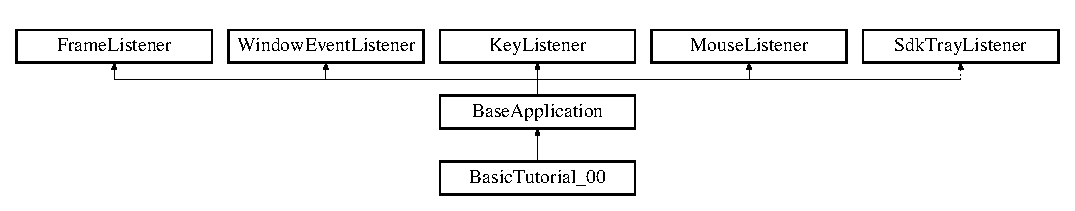
\includegraphics[height=2.000000cm]{class_base_application}
\end{center}
\end{figure}
\subsection*{Public Member Functions}
\begin{DoxyCompactItemize}
\item 
\hypertarget{class_base_application_a8a14a65a29118dd75173aa68678a05e1}{
virtual void {\bfseries go} (void)}
\label{class_base_application_a8a14a65a29118dd75173aa68678a05e1}

\end{DoxyCompactItemize}
\subsection*{Protected Member Functions}
\begin{DoxyCompactItemize}
\item 
\hypertarget{class_base_application_a5853d0e148cb85b0297a6885e1d33a89}{
virtual bool {\bfseries setup} ()}
\label{class_base_application_a5853d0e148cb85b0297a6885e1d33a89}

\item 
\hypertarget{class_base_application_a62ed46f90e9f82cc810997647a2c587e}{
virtual bool {\bfseries configure} (void)}
\label{class_base_application_a62ed46f90e9f82cc810997647a2c587e}

\item 
\hypertarget{class_base_application_ad5bc9655041e1849a4c13f444a3712bd}{
virtual void {\bfseries chooseSceneManager} (void)}
\label{class_base_application_ad5bc9655041e1849a4c13f444a3712bd}

\item 
\hypertarget{class_base_application_afa9d51527763cf9aee9cd4e1b1039d55}{
virtual void {\bfseries createCamera} (void)}
\label{class_base_application_afa9d51527763cf9aee9cd4e1b1039d55}

\item 
\hypertarget{class_base_application_aff6fd9ff1ff0978cc68f19dd65be4778}{
virtual void {\bfseries createFrameListener} (void)}
\label{class_base_application_aff6fd9ff1ff0978cc68f19dd65be4778}

\item 
\hypertarget{class_base_application_aa97beeb4059b17d0ec22eae33286ec2d}{
virtual void {\bfseries createScene} (void)=0}
\label{class_base_application_aa97beeb4059b17d0ec22eae33286ec2d}

\item 
\hypertarget{class_base_application_a365146059b25391fe400f5fdb94f011e}{
virtual void {\bfseries destroyScene} (void)}
\label{class_base_application_a365146059b25391fe400f5fdb94f011e}

\item 
\hypertarget{class_base_application_a1f8f6730cae6ec769d8730b1af48486e}{
virtual void {\bfseries createViewports} (void)}
\label{class_base_application_a1f8f6730cae6ec769d8730b1af48486e}

\item 
\hypertarget{class_base_application_ae27301702f1e5de64619a39b1929f1f9}{
virtual void {\bfseries setupResources} (void)}
\label{class_base_application_ae27301702f1e5de64619a39b1929f1f9}

\item 
\hypertarget{class_base_application_a9b77972f0f747a61e1f8ceba2ad47641}{
virtual void {\bfseries createResourceListener} (void)}
\label{class_base_application_a9b77972f0f747a61e1f8ceba2ad47641}

\item 
\hypertarget{class_base_application_aaeb764e637dd87601a81a80156659d88}{
virtual void {\bfseries loadResources} (void)}
\label{class_base_application_aaeb764e637dd87601a81a80156659d88}

\item 
\hypertarget{class_base_application_a03912a0f38b38fede7f08a2571e8fc56}{
virtual bool {\bfseries frameRenderingQueued} (const Ogre::FrameEvent \&evt)}
\label{class_base_application_a03912a0f38b38fede7f08a2571e8fc56}

\item 
\hypertarget{class_base_application_acfa977f04e435f18018ece805c1277ec}{
virtual bool {\bfseries keyPressed} (const OIS::KeyEvent \&arg)}
\label{class_base_application_acfa977f04e435f18018ece805c1277ec}

\item 
\hypertarget{class_base_application_aba5c7c9dea7a0efc58b89310bae547e5}{
virtual bool {\bfseries keyReleased} (const OIS::KeyEvent \&arg)}
\label{class_base_application_aba5c7c9dea7a0efc58b89310bae547e5}

\item 
\hypertarget{class_base_application_a126e59cb246b061e51eb6ce06a2ee8f4}{
virtual bool {\bfseries mouseMoved} (const OIS::MouseEvent \&arg)}
\label{class_base_application_a126e59cb246b061e51eb6ce06a2ee8f4}

\item 
\hypertarget{class_base_application_a9255dfc1eabefd11c474ec45a6622504}{
virtual bool {\bfseries mousePressed} (const OIS::MouseEvent \&arg, OIS::MouseButtonID id)}
\label{class_base_application_a9255dfc1eabefd11c474ec45a6622504}

\item 
\hypertarget{class_base_application_aa102c5859c14c0690c749994a446b53d}{
virtual bool {\bfseries mouseReleased} (const OIS::MouseEvent \&arg, OIS::MouseButtonID id)}
\label{class_base_application_aa102c5859c14c0690c749994a446b53d}

\item 
\hypertarget{class_base_application_afacf8a797588592ef0abbad593f10cfa}{
virtual void {\bfseries windowResized} (Ogre::RenderWindow $\ast$rw)}
\label{class_base_application_afacf8a797588592ef0abbad593f10cfa}

\item 
\hypertarget{class_base_application_ae0e37ac54a31ff6e51d58c7654ad1b90}{
virtual void {\bfseries windowClosed} (Ogre::RenderWindow $\ast$rw)}
\label{class_base_application_ae0e37ac54a31ff6e51d58c7654ad1b90}

\end{DoxyCompactItemize}
\subsection*{Protected Attributes}
\begin{DoxyCompactItemize}
\item 
\hypertarget{class_base_application_add84ba707dc6c57e6283f214b1274110}{
Ogre::Root $\ast$ {\bfseries mRoot}}
\label{class_base_application_add84ba707dc6c57e6283f214b1274110}

\item 
\hypertarget{class_base_application_a3829c6b12afe911e97e6b4524b33a38b}{
Ogre::Camera $\ast$ {\bfseries mCamera}}
\label{class_base_application_a3829c6b12afe911e97e6b4524b33a38b}

\item 
\hypertarget{class_base_application_a8a7684f4f9a57ed3089048ad1a913b2d}{
Ogre::SceneManager $\ast$ {\bfseries mSceneMgr}}
\label{class_base_application_a8a7684f4f9a57ed3089048ad1a913b2d}

\item 
\hypertarget{class_base_application_ac5d8e9c81e036897bc82f81eff8c570f}{
Ogre::RenderWindow $\ast$ {\bfseries mWindow}}
\label{class_base_application_ac5d8e9c81e036897bc82f81eff8c570f}

\item 
\hypertarget{class_base_application_a765e0df01c141a16df3178ab4f17afe6}{
Ogre::String {\bfseries mResourcesCfg}}
\label{class_base_application_a765e0df01c141a16df3178ab4f17afe6}

\item 
\hypertarget{class_base_application_a04f2fe47fa164fd78d986dc0df70b7fb}{
Ogre::String {\bfseries mPluginsCfg}}
\label{class_base_application_a04f2fe47fa164fd78d986dc0df70b7fb}

\item 
\hypertarget{class_base_application_a7faa397f4f4861ee8c361a01e90b4416}{
OgreBites::SdkTrayManager $\ast$ {\bfseries mTrayMgr}}
\label{class_base_application_a7faa397f4f4861ee8c361a01e90b4416}

\item 
\hypertarget{class_base_application_a9ae38dea6316058549151fff66a91fcd}{
OgreBites::SdkCameraMan $\ast$ {\bfseries mCameraMan}}
\label{class_base_application_a9ae38dea6316058549151fff66a91fcd}

\item 
\hypertarget{class_base_application_a6a11054ca61efdf558e0ff1b2de43a12}{
OgreBites::ParamsPanel $\ast$ {\bfseries mDetailsPanel}}
\label{class_base_application_a6a11054ca61efdf558e0ff1b2de43a12}

\item 
\hypertarget{class_base_application_ac7e861799862cb645f1d78b170aef80d}{
bool {\bfseries mCursorWasVisible}}
\label{class_base_application_ac7e861799862cb645f1d78b170aef80d}

\item 
\hypertarget{class_base_application_a755f26d3a9915aaf830750d877e39d86}{
bool {\bfseries mShutDown}}
\label{class_base_application_a755f26d3a9915aaf830750d877e39d86}

\item 
\hypertarget{class_base_application_abc9503c8462e225b5d0d55c952d9e4a9}{
OIS::InputManager $\ast$ {\bfseries mInputManager}}
\label{class_base_application_abc9503c8462e225b5d0d55c952d9e4a9}

\item 
\hypertarget{class_base_application_add9b97fbe64da2814d3af113bac58c43}{
OIS::Mouse $\ast$ {\bfseries mMouse}}
\label{class_base_application_add9b97fbe64da2814d3af113bac58c43}

\item 
\hypertarget{class_base_application_a9d6e19cf50c47379fbaae55bff28079c}{
OIS::Keyboard $\ast$ {\bfseries mKeyboard}}
\label{class_base_application_a9d6e19cf50c47379fbaae55bff28079c}

\end{DoxyCompactItemize}


The documentation for this class was generated from the following files:\begin{DoxyCompactItemize}
\item 
D:/wingo/teaching\_\-course\_\-2011/3DGameProgramming/source\_\-code/3DGame\_\-Ogre\_\-vc\_\-9\_\-v1-\/7-\/1\_\-Assigns/programs\_\-beginner/Assign\_\-01\_\-MultiViewports/source/BaseApplication.h\item 
D:/wingo/teaching\_\-course\_\-2011/3DGameProgramming/source\_\-code/3DGame\_\-Ogre\_\-vc\_\-9\_\-v1-\/7-\/1\_\-Assigns/programs\_\-beginner/Assign\_\-01\_\-MultiViewports/source/BaseApplication.cpp\end{DoxyCompactItemize}

\hypertarget{class_basic_tutorial__00}{}\section{Basic\+Tutorial\+\_\+00 Class Reference}
\label{class_basic_tutorial__00}\index{Basic\+Tutorial\+\_\+00@{Basic\+Tutorial\+\_\+00}}
Inheritance diagram for Basic\+Tutorial\+\_\+00\+:\begin{figure}[H]
\begin{center}
\leavevmode
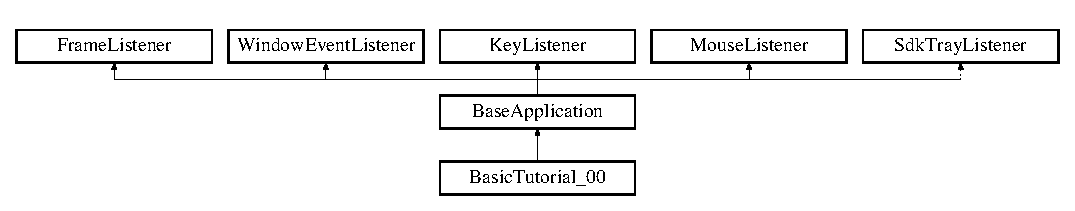
\includegraphics[height=2.382979cm]{class_basic_tutorial__00}
\end{center}
\end{figure}
\subsection*{Public Member Functions}
\begin{DoxyCompactItemize}
\item 
\mbox{\Hypertarget{class_basic_tutorial__00_a15a3d4673724ec99077ce992f996a550}\label{class_basic_tutorial__00_a15a3d4673724ec99077ce992f996a550}} 
virtual void {\bfseries create\+Scene} (void)
\end{DoxyCompactItemize}
\subsection*{Protected Member Functions}
\begin{DoxyCompactItemize}
\item 
\mbox{\Hypertarget{class_basic_tutorial__00_a0593b0fa18b690e666b042b83070606b}\label{class_basic_tutorial__00_a0593b0fa18b690e666b042b83070606b}} 
void {\bfseries resolve\+Collision} ()
\item 
\mbox{\Hypertarget{class_basic_tutorial__00_aab1bc1d4f0ade984775b3ed651f50d6f}\label{class_basic_tutorial__00_aab1bc1d4f0ade984775b3ed651f50d6f}} 
void {\bfseries resolve\+Collision\+Small\+Robots} ()
\item 
\mbox{\Hypertarget{class_basic_tutorial__00_afcf0ce12665cb66ae331dbc1eb86623d}\label{class_basic_tutorial__00_afcf0ce12665cb66ae331dbc1eb86623d}} 
void {\bfseries resolve\+Collision\+Small\+Big\+Robots} ()
\item 
\mbox{\Hypertarget{class_basic_tutorial__00_aba9704bd07c50cddf66ed6bd636fe8e2}\label{class_basic_tutorial__00_aba9704bd07c50cddf66ed6bd636fe8e2}} 
void {\bfseries resolve\+Collision\+Small\+Sphere} ()
\item 
\mbox{\Hypertarget{class_basic_tutorial__00_a719fdfadd2a46df860a34b0063a3212b}\label{class_basic_tutorial__00_a719fdfadd2a46df860a34b0063a3212b}} 
void {\bfseries resolve\+Collision\+Big\+Sphere} ()
\item 
\mbox{\Hypertarget{class_basic_tutorial__00_a3f092adc75caa10710637e11aacb96bd}\label{class_basic_tutorial__00_a3f092adc75caa10710637e11aacb96bd}} 
void {\bfseries resolve\+Collision} (Scene\+Node $\ast$nodeA, Scene\+Node $\ast$nodeB, float rA, float rB)
\item 
\mbox{\Hypertarget{class_basic_tutorial__00_a7b4f8a8aac63c3bd9b6b332077694671}\label{class_basic_tutorial__00_a7b4f8a8aac63c3bd9b6b332077694671}} 
void {\bfseries resolve\+Collision} (Scene\+Node $\ast$nodeA, Scene\+Node $\ast$nodeB, float rA, float rB, float wA, float wB)
\end{DoxyCompactItemize}
\subsection*{Protected Attributes}
\begin{DoxyCompactItemize}
\item 
\mbox{\Hypertarget{class_basic_tutorial__00_a4ce11b746634fb2edeb80c145d91d842}\label{class_basic_tutorial__00_a4ce11b746634fb2edeb80c145d91d842}} 
Scene\+Node $\ast$ {\bfseries m\+Scene\+Node} \mbox{[}1024\mbox{]}
\item 
\mbox{\Hypertarget{class_basic_tutorial__00_a4457f00e95bd513d333a9abe6a0e8291}\label{class_basic_tutorial__00_a4457f00e95bd513d333a9abe6a0e8291}} 
Entity $\ast$ {\bfseries m\+Entity} \mbox{[}1024\mbox{]}
\item 
\mbox{\Hypertarget{class_basic_tutorial__00_a6676a92b50e9b43634d4c66488537b73}\label{class_basic_tutorial__00_a6676a92b50e9b43634d4c66488537b73}} 
Ogre\+::\+Viewport $\ast$ {\bfseries m\+Viewport\+Arr} \mbox{[}8\mbox{]}
\item 
\mbox{\Hypertarget{class_basic_tutorial__00_af8d457d912286a98c0975c52d4faf910}\label{class_basic_tutorial__00_af8d457d912286a98c0975c52d4faf910}} 
Ogre\+::\+Camera $\ast$ {\bfseries m\+Camera\+Arr} \mbox{[}8\mbox{]}
\item 
\mbox{\Hypertarget{class_basic_tutorial__00_a603779b6087698c57b7989e16d8a9b93}\label{class_basic_tutorial__00_a603779b6087698c57b7989e16d8a9b93}} 
Ogre\+::\+Scene\+Manager $\ast$ {\bfseries m\+Scene\+Mgr\+Arr} \mbox{[}8\mbox{]}
\end{DoxyCompactItemize}


The documentation for this class was generated from the following files\+:\begin{DoxyCompactItemize}
\item 
3\+D\+G\+P\+\_\+201709\+\_\+02\+\_\+\+Control\+Characters\+\_\+\+Template/source/Tutorial\+Application.\+h\item 
3\+D\+G\+P\+\_\+201709\+\_\+02\+\_\+\+Control\+Characters\+\_\+\+Template/source/Tutorial\+Application.\+cpp\end{DoxyCompactItemize}

\hypertarget{class_selection_rectangle}{}\section{Selection\+Rectangle Class Reference}
\label{class_selection_rectangle}\index{Selection\+Rectangle@{Selection\+Rectangle}}
Inheritance diagram for Selection\+Rectangle\+:\begin{figure}[H]
\begin{center}
\leavevmode
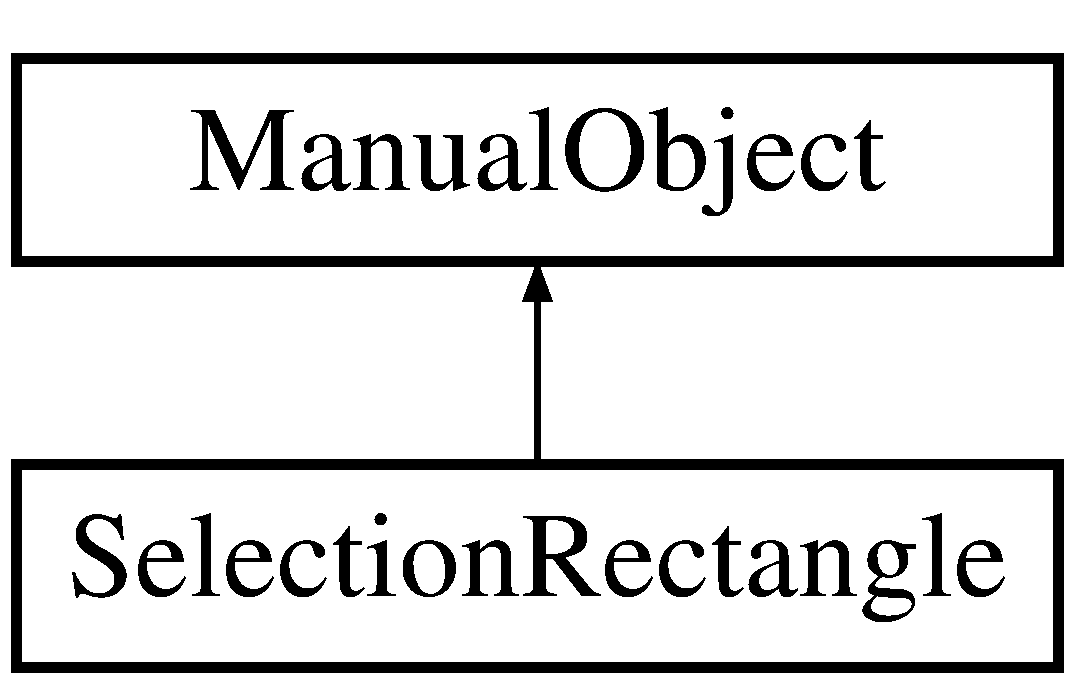
\includegraphics[height=2.000000cm]{class_selection_rectangle}
\end{center}
\end{figure}
\subsection*{Public Member Functions}
\begin{DoxyCompactItemize}
\item 
\mbox{\Hypertarget{class_selection_rectangle_a0f65ff3b042ba0163ab66fad82540420}\label{class_selection_rectangle_a0f65ff3b042ba0163ab66fad82540420}} 
{\bfseries Selection\+Rectangle} (const String \&name)
\item 
\mbox{\Hypertarget{class_selection_rectangle_a89a4528287559860ed9f2a3e6152f275}\label{class_selection_rectangle_a89a4528287559860ed9f2a3e6152f275}} 
void {\bfseries set\+Corners} (float left, float top, float right, float bottom)
\end{DoxyCompactItemize}


The documentation for this class was generated from the following file\+:\begin{DoxyCompactItemize}
\item 
3\+D\+G\+P\+\_\+201709\+\_\+02\+\_\+\+Control\+Characters\+\_\+\+Template/source/selection\+\_\+rectangle.\+h\end{DoxyCompactItemize}

\hypertarget{class_s_o_u_n_d}{}\section{S\+O\+U\+ND Class Reference}
\label{class_s_o_u_n_d}\index{S\+O\+U\+ND@{S\+O\+U\+ND}}
\subsection*{Public Member Functions}
\begin{DoxyCompactItemize}
\item 
\mbox{\Hypertarget{class_s_o_u_n_d_a7ceb7063b1ac86fadccccce1e60a70ec}\label{class_s_o_u_n_d_a7ceb7063b1ac86fadccccce1e60a70ec}} 
bool {\bfseries set\+File\+Name} (char $\ast$a\+\_\+\+File\+Name)
\item 
\mbox{\Hypertarget{class_s_o_u_n_d_a9874a1ab004717156585656243974bc9}\label{class_s_o_u_n_d_a9874a1ab004717156585656243974bc9}} 
bool {\bfseries init} ()
\item 
\mbox{\Hypertarget{class_s_o_u_n_d_a9fba48663d11f72d78d1522eea1f4f13}\label{class_s_o_u_n_d_a9fba48663d11f72d78d1522eea1f4f13}} 
bool {\bfseries play} ()
\item 
\mbox{\Hypertarget{class_s_o_u_n_d_a27cd0def63ebcede4c9820ac7a2bf2c8}\label{class_s_o_u_n_d_a27cd0def63ebcede4c9820ac7a2bf2c8}} 
bool {\bfseries is\+Stopped} () const
\end{DoxyCompactItemize}
\subsection*{Protected Attributes}
\begin{DoxyCompactItemize}
\item 
\mbox{\Hypertarget{class_s_o_u_n_d_af29fd285dd664a2824589a6b0432c722}\label{class_s_o_u_n_d_af29fd285dd664a2824589a6b0432c722}} 
A\+Luint {\bfseries ui\+Buffers} \mbox{[}N\+U\+M\+B\+U\+F\+F\+E\+RS\mbox{]}
\item 
\mbox{\Hypertarget{class_s_o_u_n_d_a5d7967b5208477b374a3880ae26ab77a}\label{class_s_o_u_n_d_a5d7967b5208477b374a3880ae26ab77a}} 
A\+Luint {\bfseries ui\+Source}
\item 
\mbox{\Hypertarget{class_s_o_u_n_d_aa96a13b3b3cc7526801488789bf92cde}\label{class_s_o_u_n_d_aa96a13b3b3cc7526801488789bf92cde}} 
A\+Luint {\bfseries ui\+Buffer}
\item 
\mbox{\Hypertarget{class_s_o_u_n_d_a43be97d9ac6fd19cf7699ef9f5afbc70}\label{class_s_o_u_n_d_a43be97d9ac6fd19cf7699ef9f5afbc70}} 
A\+Lint {\bfseries i\+State}
\item 
\mbox{\Hypertarget{class_s_o_u_n_d_aa1d2c5db17651bd6cc2af4b8d076716f}\label{class_s_o_u_n_d_aa1d2c5db17651bd6cc2af4b8d076716f}} 
C\+Waves $\ast$ {\bfseries p\+Wave\+Loader}
\item 
\mbox{\Hypertarget{class_s_o_u_n_d_aaf68e1f37c49cb40b7a61a4880aecebf}\label{class_s_o_u_n_d_aaf68e1f37c49cb40b7a61a4880aecebf}} 
W\+A\+V\+E\+ID {\bfseries Wave\+ID}
\item 
\mbox{\Hypertarget{class_s_o_u_n_d_a2e69888846a58ab6f46dad631dedea47}\label{class_s_o_u_n_d_a2e69888846a58ab6f46dad631dedea47}} 
A\+Lint {\bfseries i\+Loop}
\item 
\mbox{\Hypertarget{class_s_o_u_n_d_afef36da1f658dfe7f616c1bba79d3590}\label{class_s_o_u_n_d_afef36da1f658dfe7f616c1bba79d3590}} 
A\+Lint {\bfseries i\+Buffers\+Processed}
\item 
\mbox{\Hypertarget{class_s_o_u_n_d_a41a714322ff9041ccad9086d5cb01402}\label{class_s_o_u_n_d_a41a714322ff9041ccad9086d5cb01402}} 
A\+Lint {\bfseries i\+Total\+Buffers\+Processed}
\item 
\mbox{\Hypertarget{class_s_o_u_n_d_aa5eef80846dd17340ba3ee615c1c7f87}\label{class_s_o_u_n_d_aa5eef80846dd17340ba3ee615c1c7f87}} 
A\+Lint {\bfseries i\+Queued\+Buffers}
\item 
\mbox{\Hypertarget{class_s_o_u_n_d_aa617757733d08fb0c90e2aee02c67ef0}\label{class_s_o_u_n_d_aa617757733d08fb0c90e2aee02c67ef0}} 
W\+A\+V\+E\+F\+O\+R\+M\+A\+T\+EX {\bfseries wfex}
\item 
\mbox{\Hypertarget{class_s_o_u_n_d_abccb3cdff4440d791c9a2e3fbc77b77c}\label{class_s_o_u_n_d_abccb3cdff4440d791c9a2e3fbc77b77c}} 
unsigned long {\bfseries ul\+Data\+Size}
\item 
\mbox{\Hypertarget{class_s_o_u_n_d_aba5b5324724cb90d8aa3f9d31069ba76}\label{class_s_o_u_n_d_aba5b5324724cb90d8aa3f9d31069ba76}} 
unsigned long {\bfseries ul\+Frequency}
\item 
\mbox{\Hypertarget{class_s_o_u_n_d_ab9858c7e9e36af3bf8c4d0e76c13718c}\label{class_s_o_u_n_d_ab9858c7e9e36af3bf8c4d0e76c13718c}} 
unsigned long {\bfseries ul\+Format}
\item 
\mbox{\Hypertarget{class_s_o_u_n_d_a49925a922bdd7062fc9916fd86254980}\label{class_s_o_u_n_d_a49925a922bdd7062fc9916fd86254980}} 
unsigned long {\bfseries ul\+Buffer\+Size}
\item 
\mbox{\Hypertarget{class_s_o_u_n_d_a3af2648bc0569915511860ebebfcd246}\label{class_s_o_u_n_d_a3af2648bc0569915511860ebebfcd246}} 
unsigned long {\bfseries ul\+Bytes\+Written}
\item 
\mbox{\Hypertarget{class_s_o_u_n_d_a46832ac27ae2ef80a8696d23a3d7acff}\label{class_s_o_u_n_d_a46832ac27ae2ef80a8696d23a3d7acff}} 
void $\ast$ {\bfseries p\+Data}
\item 
\mbox{\Hypertarget{class_s_o_u_n_d_a23db6da1d79da30db5f1697d9cbea68b}\label{class_s_o_u_n_d_a23db6da1d79da30db5f1697d9cbea68b}} 
char $\ast$ {\bfseries m\+File\+Name}
\end{DoxyCompactItemize}


The documentation for this class was generated from the following files\+:\begin{DoxyCompactItemize}
\item 
3\+D\+G\+P\+\_\+201709\+\_\+02\+\_\+\+Control\+Characters\+\_\+\+Template/source/sound.\+h\item 
3\+D\+G\+P\+\_\+201709\+\_\+02\+\_\+\+Control\+Characters\+\_\+\+Template/source/sound.\+cpp\end{DoxyCompactItemize}

%--- End generated contents ---

% Index
\backmatter
\newpage
\phantomsection
\clearemptydoublepage
\addcontentsline{toc}{chapter}{Index}
\printindex

\end{document}
